%-------------------------------------------------------------------------------
\section{Scalability of the Packrat Proxy}
\label{sec:eack}
%-------------------------------------------------------------------------------
An on-path proxy handles many tens to hundreds of thousands of concurrent connections at once.
Any per-packet overhead incurred by the \Sys protocol at the proxy must be
extremely small. The \Sys proxy encodes every packet in the base connection and, unlike
the Sidekick proxy, also decodes every acknowledgment
($91\!\times$ more expensive than encoding in \cite{yuan2024sidekick}).
We want to explore whether a different type of acknowledgment of encrypted packets
can be more suitable in the setting of in-network
retransmissions for its computational efficiency.

The problem of providing a concise acknowledgment of encrypted packet identifiers
boils down to a more general problem called set reconciliation. In this problem,
two parties, each with a set, learn the items missing in the other
set~\cite{minsky2003set,eppstein2011straggler}.
There are two well-known solutions with different tradeoffs. The quACK
applies the space-optimal deterministic solution based on
power sum polynomials, which is easy to reason about for correctness~\cite{yuan2024sidekick}.
Other work applies the probabilistic Bloom filter solution
for its computational efficiency~\cite{yang2024practical,summermatter2021byzantine},
which inspires our construction of the eACK.


% In particular, we want to improve the computational efficiency of decoding
% (a $91\!\times$ more expensive operation than encoding in the power sum quACK),
% since it now incurs a per-packet overhead at the proxy compared to the Sidekick protocol,

% \thea{Emphasize here the key diff from basic connection splitters -- it's the encoding and decoding}

% \thea{For decoding, need to motivate why we know that decoding is expensive specifically.}

% \thea{I find this paragraph confusing in both the description of the problem
% and what prior work it's referring to.}
% Prior work on the \textit{(sub)set reconciliation problem}, where two parties
% each with a set learn the $m$ items missing from the subset, provides useful
% context on how to optimize these operations~\cite{eppstein2011straggler}.
% There are two main classes of solutions in prior work.
%  \thea{need to intro the power sum quack and how it was applied by your NSDI paper -
%  otherwise the transition to IBLT doesn't make sense.}
% The power sum quACK applies the
% space-optimal, deterministic solution and encodes the set as the first $m$
% power sum symmetric polynomials. Can we also apply the other solution and encode
% the set in a probabilistic Bloom Filter?
% \thea{I think this last sentence is abrupt}

% \thea{Again, I think there needs to be more motivation behind exploring IBLT quacks
% and some reference to (your) prior work that applied the power sum quack}

Set reconciliation with a Bloom filter has mainly been applied to large distributed systems~\cite
{yang2024practical,summermatter2021byzantine}. However, in the \Sys setting
where items are network packets, the encoding must must fit in a typical packet
MTU of 1500 bytes, and decoding must complete in millisecond RTT timescales or
less. We discuss the nuances of using the IBLT at a small granularity, and
also explore the tradeoffs of the eACK compared to the quACK.

Another way to reduce the impact of decoding at the proxy is simply to send smaller
and fewer eACKs. When the eACK sender is at the proxy, such as in Sidekick,
it doesn't have much flexibility in changing how often it eACKs given
the base protocol is completely opaque. But when the eACK sender is co-located
with an application endpoint, the endpoint can leverage its knowledge about the
base acknowledgment scheme to dynamically adjust the eACK.
We describe two optimizations: \textit{rateless eACKs} and \textit{selective eACKing}.

% \thea{This last part isn't really about decoding. Maybe make section about load on proxy,
% then go decoding (motivate why the focus on decoding) --> reducing load. can name that
% connection management is out of scope for this section because it's the same as
% connection splitters and is evaluated later.}

\begin{lstfloat}[t]
\begin{lstlisting}[language=Rust]
trait quACKK {
    fn count() -> usize;
    fn last_identifier() -> u32;
    fn encode(item: u32);
    fn remove(item: u32);
    fn sub(rhs: quACKK) -> quACKK;
    fn decode() -> &[u32];
}
\end{lstlisting}
\captionof{lstlisting}{Pseudocode interface for the implementation of the quACKK
 in the \texttt{quack} library. Each item is a 4-byte random identifier
 referring to a network packet.}
\label{lst:quack-interface}
\end{lstfloat}


\subsection{IBLT Acknowledgment}
\label{sec:eack:iblt}

In this section, we apply
the Rateless Invertible Bloom Lookup Table~\cite{yang2024practical}
to describe a new probabilistic construction of an acknowledgment
for encrypted packets. We describe its data structure and implementation
and formalize an interface for these acknowledgments in \Cref{lst:quack-interface}.

\paragraph{Rateless IBLT crash course.} The IBLT is like the final boss version
 of the Bloom filter~\cite{goodrich2011invertible}. The data structure consists of $t$ cells. Each
 cell is represented by an XOR and a count of items in the cell. A
 deterministic hash function maps each item to a small number of randomly
 distributed cells. The Rateless IBLT presents a novel pseudorandom mapping
 algorithm that maps an item to $O(\log(t))$ cells, with greater density in
 cells with smaller indexes~\cite{yang2024practical}. We leverage this
 efficient mapping and its rateless properties in the eACK.

The IBLT allows the insertion and deletion of items. To find the set difference
between the items in two IBLTs, we first ``subtract'' the corresponding XORs
and counts. Then we decode the items in the difference IBLT by deleting items
from cells with a count of 1 or -1 until no such cells remain. Decoding is
successful if all counts and XORs are 0 at the end, and can fail
probabilistically due to hash collisions.

% \paragraph{Data structure.} The fields in the IBLT eACK are similar: a 4-byte
% count of received elements, a $4$-byte identifier of the last packet
% received, and then $t$ coded symbols. However, each coded symbol instead of
% being a power sum, is an XOR of packet identifiers mapped to that cell as
% well as an $1$-byte count.

% The number of coded symbols maintained at the endpoint and proxy are
% pre-determined. In the case of the IBLT eACK, we generally need some
% constant factor more symbols than the threshold number of missing packets to
% decode those packets. Otherwise, the fields of the data structure are pretty
% similar, with different implementations for the function interface.

\paragraph{Data structure.}


The eACK implements
the interface defined in \Cref{lst:quack-interface} and makes direct use of the Rateless IBLT.
The \texttt{encode()} and \texttt{remove()} functions implement IBLT insertion
and deletion, while \texttt{sub()} and \texttt{decode()} implement
the decoding process of the difference IBLT.
Each item in the encoding is a 4-byte identifier referring to a packet. The
identifier is specified by a fixed offset into the randomly encrypted packet
payload. Each \texttt{Symbol} (\Cref{fig:payloads:client}) corresponds to a
cell, containing an XOR of 4-byte identifiers and a count.

The main advantage of the eACK is the computational complexity of its
operations (\Cref{tab:quack-complexity}). Unlike the quACK,
which encodes each item in all $t$ symbols, the eACK only uses
$O(\log(t))$ symbols, making both encoding and decoding more efficient.

\begin{table}[t]
    \centering
    \begin{tabular}{r l l}
        \toprule
        \bf & Power Sum~\cite{yuan2024sidekick} & IBLT \\
        \midrule
        Encode & $O(t)$ & $O(\log(t))$ \\
        Decode & $O(Nt)$ & $O(m\log(t))$ \\
        $t=$Size & $O(m)$ & $O(m)$ \\
        \bottomrule
    \end{tabular}
    \caption{The computational complexity of the encoding and decoding
    operations of each type of eACK, and the number of symbols. The IBLT
    is theoretically better or the same in all regards, but it
    incurs constant overheads in the size and in hashing.
    $N$ is the number of packets at the proxy, $m < N$ is the number of
     missing packets, and $t$ is the number of symbols.}
    \label{tab:quack-complexity}
\end{table}

\paragraph{Serialization in a packet MTU.} The main disadvantage of the IBLT in
 the \Sys setting is its size in practice. The IBLT typically requires a constant factor
 more symbols than the number of items in the set to decode the set without a
 collision. Compared to power sums, each symbol also requires a count. While
 these constant factors are inconsequential in larger distributed systems,
 which reconcile larger sets with encodings much larger than an MTU, they
 matter here.

We carefully selected the bit widths for each field. Note that each eACK needs
to fit in a single UDP datagram, which limits us to $\approx\!1400$ bytes
excluding headers. If each XOR is $4$ bytes, then there can be at most $350$
packets in the set difference. Note that $8$-byte identifiers are unnecessary
because collisions are unlikely in these small set difference sizes. The count
in each symbol needs to be as large as the set difference size. It can also be
an unsigned integer because we do subset (and not set) reconciliation, and we
can subtract with overflow. An 8-bit integer goes up to $255$, which is
sufficiently close. Thus the largest eACK contains $255$ symbols or $4 +
4 + 255 \cdot 5 = 1283$ bytes in the \texttt{eACK} payload.

% If computation matters more than link overheads and occasional failure, can
% there be a version of a quACK that uses the IBLT? The rateless feature does
% not really apply here because since round-trips are costly for the short
% feedback loop of the sidekick protocol.

\subsection{IBLT vs. Power Sum Microbenchmarks}
\label{sec:eack:microbenchmarks}

Both the IBLT and power sums are derived from set reconciliation
techniques, so when should we prefer one to the other?
We adapt the power sum quACK from \cite{yuan2024sidekick} for the interface
in \Cref{lst:quack-interface}
so that they can be used interchangeably in our microbenchmarks and compare
it to our implementation of the IBLT eACK.
In this section, we compare the overheads in practice.
We run the microbenchmarks on a single core of an AWS m4.xlarge instance.

\paragraph{Encoding.}

% The computational complexity of encoding is more efficient in the IBLT than
% power sums, updating only $O(\log(t))$ symbols instead of all $t$ (\Cref
% {tab:quack-complexity}).
Encoding in the IBLT is faster in practice when there are at least
$\approx\!30$ symbols (\Cref{fig:quack:encode}).
Each update in the IBLT uses an expensive square root instruction in the
pseudorandom mapping algorithm, adding constant factor overheads that impact
smaller numbers of symbols.

\paragraph{Decoding.}

% Decoding is also more efficient in computational complexity in the IBLT (\Cref
% {tab:quack-complexity}).
Decoding in the IBLT is much faster in practice for any number of symbols
(\Cref{fig:quack:decode}). Note that the power sum quACK actually uses a decoding
method that is linear in \textit{all} packets received, not just the \textit
{missing} packets, due to the complexity of symmetric polynomial
factorization.

\begin{figure}[t]
    \centering
    \begin{subfigure}[b]{0.49\linewidth}
        \centering
        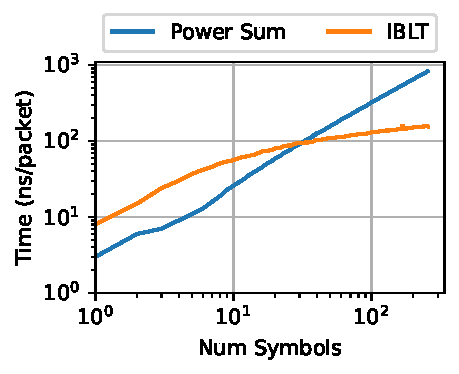
\includegraphics[width=\linewidth]{quack/figures/quack_encode.pdf}
        \caption{Encode time.}
        \label{fig:quack:encode}
    \end{subfigure}
    \begin{subfigure}[b]{0.49\linewidth}
        \centering
        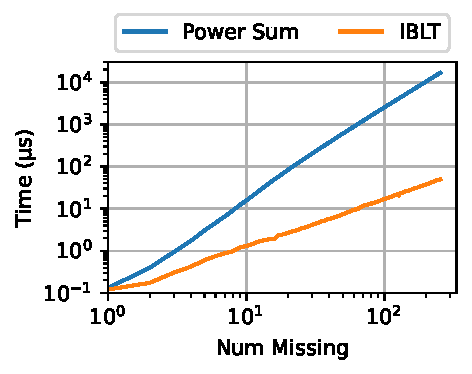
\includegraphics[width=\linewidth]{quack/figures/quack_decode.pdf}
        \caption{Decode time.}
        \label{fig:quack:decode}
    \end{subfigure}
    \caption{IBLT vs. power sum quACK microbenchmarks. The number of trials is
     such that the cumulative time is at least $100$ ms. With rateless quACKs,
     the client can encode much larger numbers of symbols $t$ while the proxy
     decodes fewer symbols in the common case.
     % The logscale axes emphasize the overheads at smaller numbers.
     }
    \label{fig:quack}
\end{figure}
\begin{figure}[t]
    \centering
    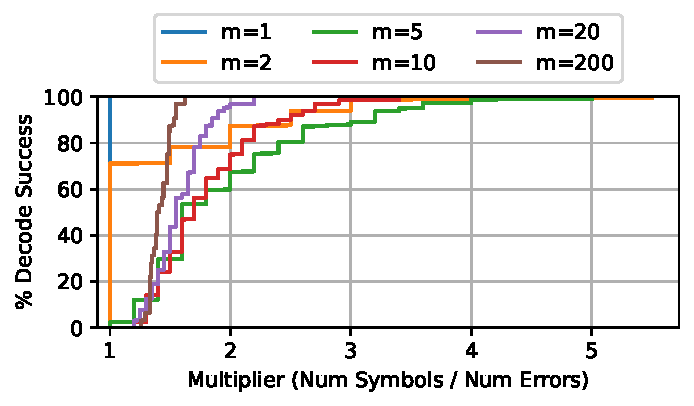
\includegraphics[width=0.9\linewidth]{packrat-paper/figures/quack_multiplier.pdf}
    \caption{The CDF of the minimum number of symbols $t$ needed to successfully
    decode an quACK for various numbers of missing packets $m$, 100000 trials.}
    \label{fig:iblt-quack}
\end{figure}

\paragraph{Non-determinism.} It is unknown
 how many symbols are required in the IBLT to decode the same number of
 $m$ missing packets using power sums in the previous benchmarks. There is a constant
 factor overhead ($1.35\times$ on average~\cite{yang2024practical}).
 \Cref{fig:iblt-quack} shows the CDF of the minimum number of symbols to decode
 various $m$ as this constant multiplier increases. $m=1$ trivially
 requires one symbol, while the multiplier decreases for higher $m$ to
 achieve the same success rates.

The eACK sender does not know how many symbols it needs to encode to later
decode a certain $m$. Using power sums, this is exactly $m$ symbols. In
the eACK, $4 \cdot m$ symbols have at least a $\!98.8\%$ success rate for
all $m$ evaluated in \Cref{fig:iblt-quack}. When $m$ is large, the eACK utilizes more
of the link, but maintaining more symbols at the proxy and client means
the \Sys has a greater worst-case tolerance for errors with the same encoding
overheads. The \Sys proxy can reset the connection if it cannot decode an eACK.

\paragraph{Summary.}

To make the IBLT data structure suitable for small, network packets, we
carefully consider constant factor overheads in the
number of symbols and the computational efficiency. We find the eACK
is most likely to be useful in settings with high, bursty loss, where
encoding and decoding large numbers of symbols is more efficient than the
quACK. However, the quACK is still more efficient when
loss is small or infrequent.
% An IBLT quACK with $100$ symbols can encode packets at $131$ $\mu$s/packet. In
% comparison, the power sum quACK can only encode with $42$ symbols in the same amount
% of time, having a lower worst-case tolerance for errors. Decoding $42$ missing
% packets takes $103$ $\mu$s in the IBLT quACK, $21\%$ faster than the power sum
% quACK.

\subsection{eACKing with Client Hints}
\label{sec:eack:hints}

We describe two optimizations at the client for dynamically adjusting the eACK
based on knowledge of the base connection to send smaller and fewer eACKs
overall.
We evaluate the impact of these optimizations in \Cref{sec:evaluation:link-overheads}.

\paragraph{Rateless eACKs.} The number of symbols in the eACK is configured
 for the worst case, but it is wasteful to consistently send hundreds of bytes
 over the wire for each eACK. Unlike set reconciliation in distributed
 systems, eACKs are transmitted at millisecond RTT timescales.

In the blockchain setting, the two parties negotiate to determine the number of
missing items, and to send additional symbols if the current number is not
enough to probabilistically decode. This minimizes the number of symbols sent
over the wire, but the in-network retransmission setting does not have the time
to negotiate over multiple RTTs. How else can we apply the rateless property to
eACKs?

In fact, the client can estimate the number of retransmissions it expects from
the proxy and send a smaller eACK, while locally encoding enough symbols for
the worst case. For example, the client can count the number of gaps in an ACK,
or the packets for which it would send a NACK. Both the IBLT and power sums
have the property that a strict prefix of symbols is sufficient to decode a
smaller error.

% We implement this in \texttt{serialize\_rateless()} (\Cref
% {lst:quack-interface}), and find that in practice this optimization
% significantly reduces link overheads while allowing the \Sys protocol to
% dynamically adjust to changing loss conditions (\Cref{sec:evaluation}).
% The client can also select the number of symbols with less precision without
% concern for the potential link overheads.

\paragraph{Selective eACKing.} If the client does not expect it needs a
 retransmission, there is not much point in sending an eACK. In NACK schemes,
 where the client detects loss and asks for a retransmission, it can choose to
 selectively eACK only when it would otherwise send a NACK. Note that the client can omit
 regular eACKs without the cache exploding in size because the proxy
 optimistically evicts packets, and these are likely to be received or the
 client would have NACKed.\\
